\documentclass{article}
\usepackage{graphicx}
\usepackage{subcaption}
\usepackage{xcolor}
\usepackage{tikz}

\begin{document}

\begin{figure*}[t]
\centering
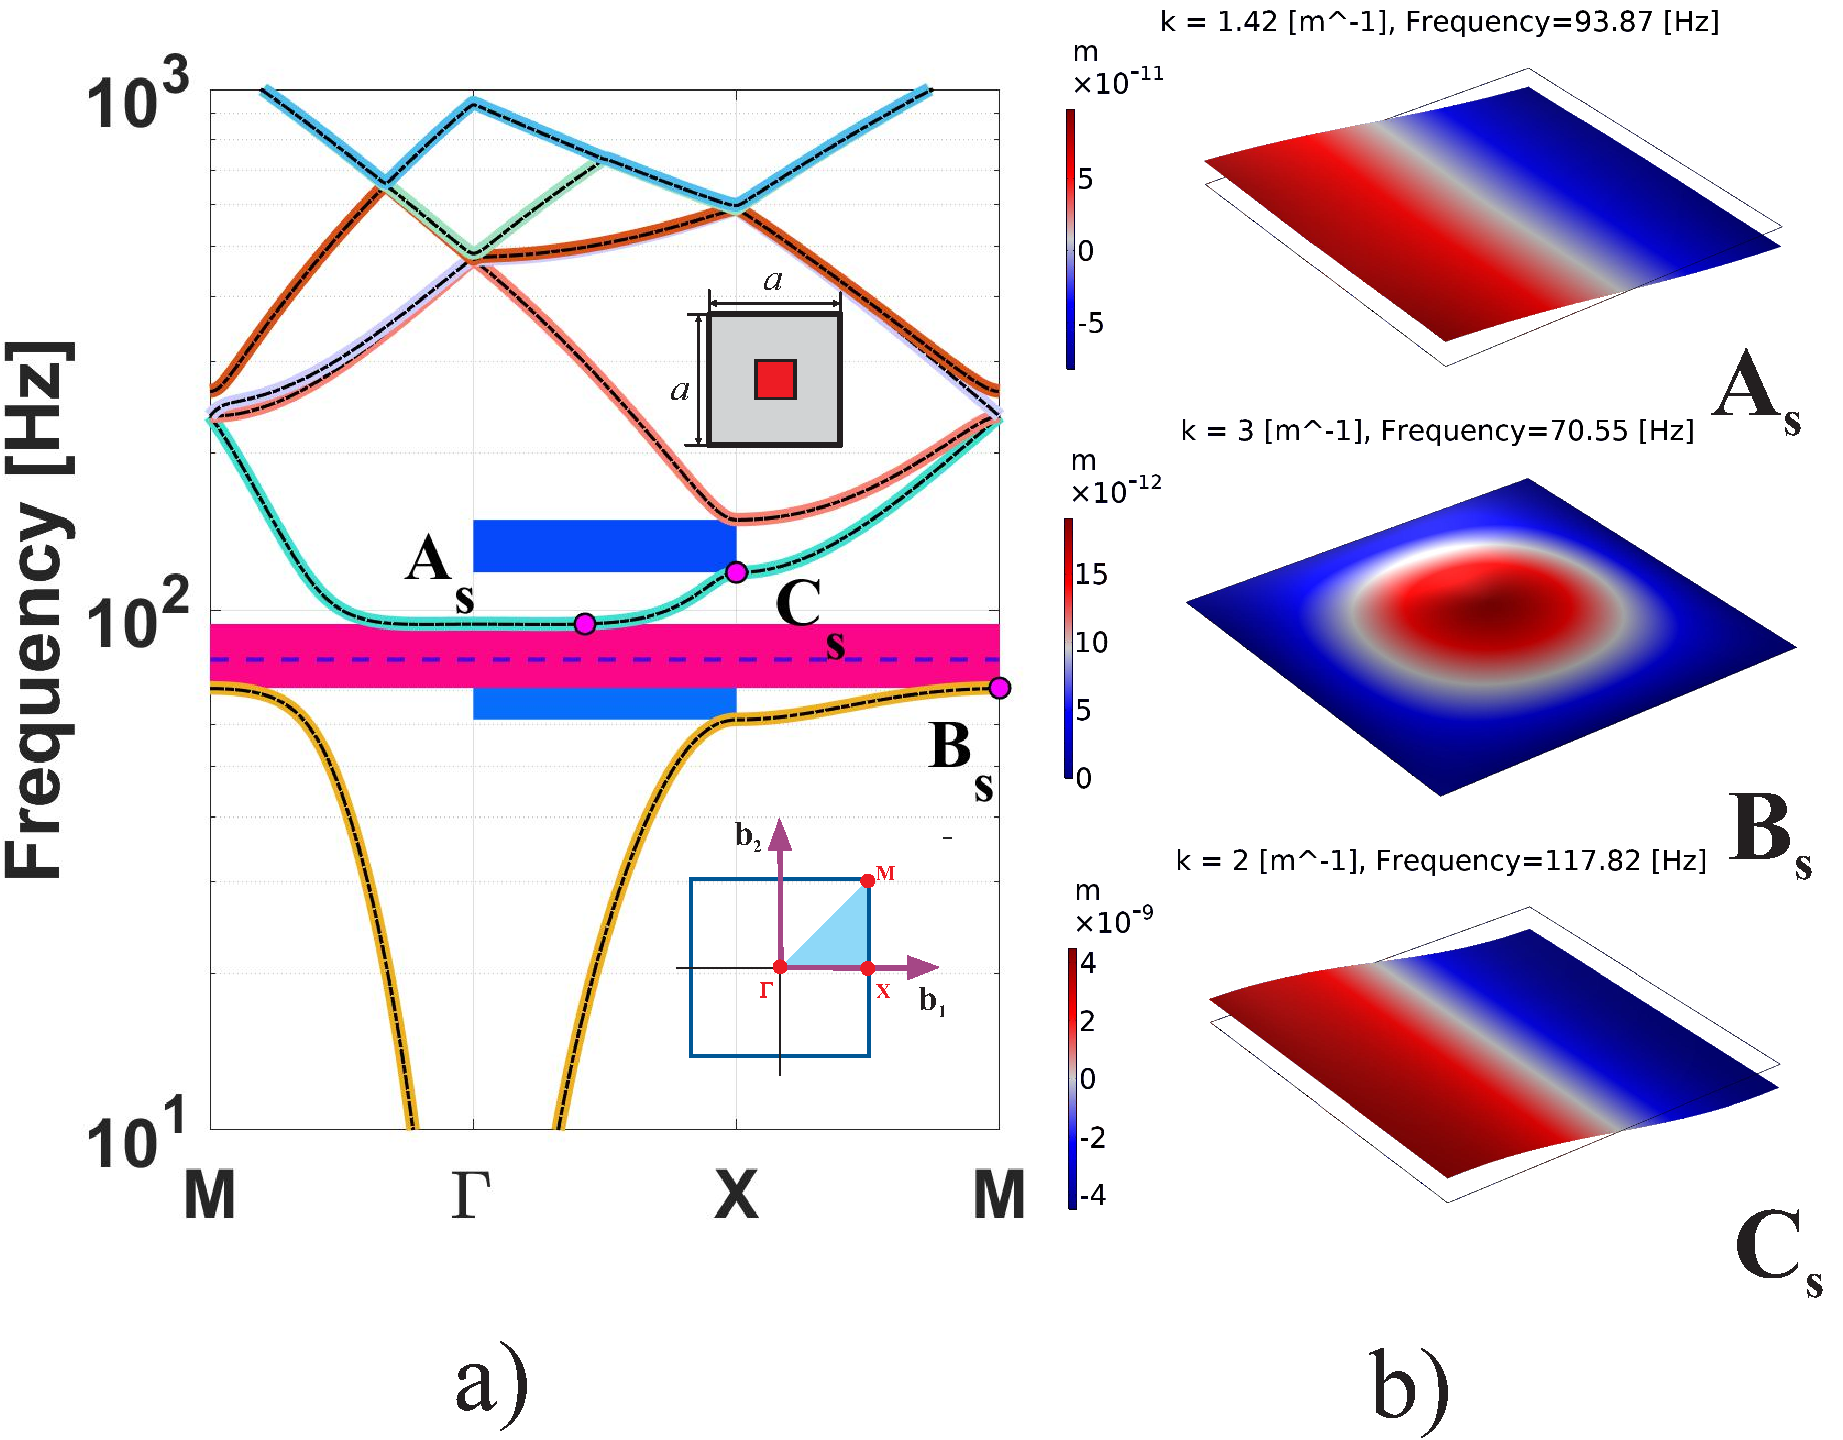
\includegraphics[width=1.0\textwidth]{1_1_disp_frf_square.pdf}

\vspace{0.3cm}

% Legenda externa compacta em formato tabular
\centering
\small
\begin{tabular}{@{}c@{\hspace{0.3em}}l@{\hspace{1.0em}}c@{\hspace{0.3em}}l@{\hspace{1.0em}}c@{\hspace{0.3em}}l@{}}
% Linha 1 - Band gaps (retângulos)
\tikz{\filldraw[cyan!70!blue] (0,0) rectangle (0.6,0.3);} & PBGW 1 - $\Gamma \rightarrow$ X &
\tikz{\filldraw[magenta!90!red] (0,0) rectangle (0.6,0.3);} & FBGW 1 &
\tikz{\filldraw[blue!80!cyan] (0,0) rectangle (0.6,0.3);} & PBGW 2 - $\Gamma \rightarrow$ X \\[0.3em]

% Linha 2 - Modos PWE
\tikz{\draw[line width=3.5pt, orange!90!yellow] (0,0.15) -- (0.6,0.15);} & K-L: Mode 1 - PWE &
\tikz{\draw[line width=3.5pt, cyan!80!white] (0,0.15) -- (0.6,0.15);} & K-L: Mode 2 - PWE &
\tikz{\draw[line width=3.5pt, red!60!black] (0,0.15) -- (0.6,0.15);} & K-L: Mode 3 - PWE \\[0.3em]

% Linha 3 - FEM e LRSC
\tikz{\draw[line width=3pt, black, dashed] (0,0.15) -- (0.6,0.15);} & K-L: Modes 1-3 - FEM &
\tikz{\draw[line width=2.5pt, blue!80!cyan, dashed] (0,0.15) -- (0.6,0.15);} & LRSC: 80 [Hz] & & \\
\end{tabular}

\caption{Band structure and wave mode shapes for a square lattice unit cell with single resonator ($f_r = 80$ Hz) in a thin plate. (\textit{a}) Dispersion diagram computed with PWE and FEM methods along M--$\Gamma$--X--M showing FBGW 1 ($f_1 = 70.72$ Hz, $f_2 = 93.88$ Hz, $\Delta f_{12} = 23.16$ Hz), PBGW 1 ($\Gamma \rightarrow$ X: $f_1 = 61.54$ Hz, $f_2 = 93.88$ Hz, $\Delta f_{12} = 32.33$ Hz), and PBGW 2 ($\Gamma \rightarrow$ X: $f_1 = 117.91$ Hz, $f_2 = 149$ Hz, $\Delta f_{12} = 31.09$ Hz). (\textit{b}) Wave mode shapes at points $A_s$, $B_s$, and $C_s$ computed by FEM.}
\label{pwe_fem_disp_modal_square}
\end{figure*}

\end{document}
